\documentclass[a4paper,10pt,twoside]{scrartcl}
% \usepackage[pdflatex, tightpage]{preview}
\usepackage[svgnames]{xcolor}
\usepackage{tikz}
\usepackage{amsmath,amsfonts}
% \usepackage{graphicx}
\usepackage[left=2cm, right=2cm, top=1.8cm]{geometry}
\usepackage{rotating}
\usepackage{fancyhdr}
\usepackage[texcoord]{eso-pic}
\usepackage[algosection]{algorithm2e}
\usepackage[pdftitle={PfTools},pdfauthor={Thierry Schuepbach},pdfsubject={PfTools},baseurl={www.sib.swiss}]{hyperref}

\usetikzlibrary{decorations.markings}
\usetikzlibrary{shapes.geometric}
\usepackage[framemethod=default]{mdframed}
\usepackage{enumerate}
\global\mdfdefinestyle{exampledefault}{%
linecolor=lightgray,linewidth=1pt,%
leftmargin=1cm,rightmargin=1cm,
}

\newenvironment{notes}{%
\vspace{0.5em}
\mdfsetup{%
frametitle={\tikz\node[fill=white,rectangle,inner sep=0pt,outer sep=0pt]{Notes};},
frametitleaboveskip=-0.5\ht\strutbox,
frametitlealignment=\raggedright
}%
\begin{mdframed}[style=exampledefault]
}{\end{mdframed}}

\pgfdeclarelayer{edgelayer}
\pgfdeclarelayer{nodelayer}
\pgfsetlayers{edgelayer,nodelayer,main}

\tikzstyle{none}=[inner sep=0pt]

\tikzstyle{rn}=[circle,fill=Red,draw=Black,line width=0.8 pt]
\tikzstyle{gn}=[circle,fill=Lime,draw=Black,line width=0.8 pt]
\tikzstyle{yn}=[circle,fill=Yellow,draw=Black,line width=0.8 pt]
\tikzstyle{newstyle}=[circle,fill=White,draw=Black,minimum width=3pt,inner sep=0pt]

\tikzstyle{simple}=[-,draw=Black,line width=2.000]
\tikzstyle{arrow}=[-,draw=Black,postaction={decorate},decoration={markings,mark=at position .5 with {\arrow{>}}},line width=2.000]
\tikzstyle{tick}=[-,draw=Black,postaction={decorate},decoration={markings,mark=at position .5 with {\draw (0,-0.1) -- (0,0.1);}},line width=2.000]
%\setlength\PreviewBorder{2mm} % use to add a border around the image

% ----------------------------------------------------------------
\vfuzz2pt % Don't report over-full v-boxes if over-edge is small
\hfuzz2pt % Don't report over-full h-boxes if over-edge is small
% MATH -----------------------------------------------------------
\newcommand{\norm}[1]{\left\Vert#1\right\Vert}
\newcommand{\abs}[1]{\left\vert#1\right\vert}
\newcommand{\set}[1]{\left\{#1\right\}}
\newcommand{\Real}{\mathbb R}
\newcommand{\eps}{\varepsilon}
\newcommand{\To}{\longrightarrow}
\newcommand{\BX}{\mathbf{B}(X)}
\newcommand{\A}{\mathcal{A}}
\renewcommand{\vec}[1]{\mathbf{#1}}
\newenvironment{alg}{\begin{algorithm} \dontprintsemicolon \SetLine
}{\end{algorithm}}
\setlength{\algomargin}{1cm}
%opening
\title{PfTools Software Suite}
\author{P. Bucher, L. Cerutti, M. Pagni, T. Schuepbach}

% Philipp Bucher
% Biocomputing Group
% Swiss Institute for Experimental Cancer Research
% 1066 Epalinges s/Lausanne
% Switzerland
% 
% Telephone: (+41 21) 692 58 92
% Electronic mail address: pbucher@isrec-sun1.unil.ch

% \Version{Version 1.3, May 1997}

\pagestyle{fancy}
\begin{document}
% Draft watermark symbol
 \AddToShipoutPicture{%
 \AtTextLowerLeft{ 
  
\includegraphics{draft2.eps}
  }
 }
 
 \renewcommand{\headheight}{30.0pt}
 \fancyhead{} % clear all fields
% \fancyhead[CO,CE]{SIB Swiss Institute of Bioinformatics \& Vital-IT Group}
 \fancyhead[LE,RO]{
\includegraphics[height=.9cm]{small_logo_sib.eps}}
 \fancyfoot[LE,RO]{\thepage}
 \fancyfoot[CO,CE]{\begin{footnotesize}\textcopyright \, 2013 SIB Swiss Institute of Bioinformatics                        
             \end{footnotesize}}
 
 \renewcommand{\headrulewidth}{0.4pt}
 \renewcommand{\footrulewidth}{0.4pt}
 
\maketitle

\begin{abstract}
  The present document gathers pieces of informations for the use of the PfTools software suite. It supersedes and extends 
  \emph{A generalized profile syntax for protein and nucleic acid sequence motifs} from Philip Bucher distributed in version earlier than 3.0.
  This document may be copied and redistributed freely, without advance permission, provided that this statement is reproduced with any copy.
  \tableofcontents
\end{abstract}
\newpage

\section*{Introduction}
\addcontentsline{toc}{section}{Introduction}
  This document describes a general syntax to express a quantitative, primary structure-based protein or nucleic acid sequence motif. The designation
  \emph{quantitative} means that a motif description assigns a degree of similarity to a potential match rather than a binary status of true or
  false. The restriction \emph{primary structure-based} implies that the probability of finding a specific residue at one position is independent of any
  residue occurring at another position.

  The generalised profile syntax has been designed for and will be used in future releases of the PROSITE data bank. In addition, it will be used in
  a similar data bank of nucleic acid sequence motifs currently under development by the author. Other researchers working on sequence motifs
  are encouraged to use the same format for their own motif collections, and may include this document in a public distribution release.

  The term \emph{generalised profile syntax} is meant to indicate that the proposed data structure represents a generalisation of the profile type
  described by Gribskov et al. \cite{Gribskov90}. However, similar motif descriptors have been introduced by others under different names, e.g. weight matrices \cite{Staden90}
  or flexible patterns \cite{Barton90}.\\
  The following terminology is adopted in this document:
 \begin{itemize}
  \item The term \emph{profile} refers to a quantitative motif description based on the generalised profile syntax.
  \item The term \emph{pattern} refers to a qualitative motif description based on a regular expression-like syntax such as the one currently used in 
	PROSITE entries marked as \textbf{PATTERN}.
  \item The term \emph{motif} refers to the biological object one attempts to approximate by a pattern or a profile.
 \end{itemize}
  Note that the PROSITE data bank reserves the token \textbf{MATRIX} to identify entries containing profiles.
  

  
  The design of the new profile structure has been guided by various biological and technical considerations. High priority has been given to the
  following principles:
  \begin{enumerate}[(A)]
    \item Syntactic versatility

      The syntax should be versatile enough to cover a large variety of biologically relevant motifs. In particular, it should be be possible to accu-
      rately represent the following objects:
      \begin{itemize}
	\item Signatures for various types and levels of protein taxons.
	\item Highly degenerate protein structural and functional domains such as the immunoglobulin domains, or the SH2 and SH3 domains.
	\item Consensus sequences of interspersed repetitive DNA elements (SINEs and LINEs).
	\item Basic gene expression signals, e.g. promoter elements, RNA processing signals, translational initiation sites.
	\item Recognition motifs of a large variety of sequence-specific DNA-binding proteins.
	\item Protein and nucleic acid compositional domains, e.g. glutamine-rich activation domains, CpG islands.
      \end{itemize}

    \item Determinative search instructions

      The profile syntax should have the capacity to encode precise and complete instructions for a motif search. Ideally, the result of a motif search
      should be determined by the profile and a sequence alone, i.e. not depend on parameters of the search method. In practice, this goal may only be 
      approximately achieved due to ambiguities arising with multiple locally optimal profile-sequence alignments (see Section \ref{Profile accessories}).

      \begin{notes}
      \begin{itemize}
	\item In other implementations of similar methods, e.g. GCG profiles or HMMER
	Hidden Markov models software, different search methods are available as options and parameters of the search programs rather than as syntactic
	features of the motif description itself. For the profiles in PROSITE, inclusion of determinative search instructions is a necessity because 
	otherwise the information given on the \textbf{NR} lines (statistics of true and false positives/negatives) would have no meaning.
	\item The notion of determinative search instructions is not meant to imply a specific search algorithm.  There is space for different technical
	solutions to achieve the same result.
      \end{itemize}
      \end{notes}
  
    \item Openness to different interpretations

      A profile syntax is situated at the interface between a motif definition and a motif search method. As such it can serve as a melting pot for
      integrating complementary efforts. While a rigid meaning vis-a-vis a search method is desirable, flexibility with regard to motif definition
      methods is equally important. In order to achieve such flexibility, it is essential that the profile parameters remain open to a variety of different
      theoretical interpretations implicit in different methodologies.

      Relevant motif definition techniques may include both comparative structural and wet biochemical approaches. It is thus conceivable that the
      same type of numeric profile parameter may reflect log-probabilities in
      one case, and binding energies in another. A profile syntax must be neutral in this respect in order to be generally acceptable to a heterogeneous
      research community relying on different rationales for motif definition.

    \item Compatibility with existing search methods

      As a profile is required to encode determinative directives for a motif search, the underlying syntax should have the capacity to emulate most of
      the commonly used motif search techniques, such as:
      \begin{itemize}
	\item Search for PROSITE patterns.
	\item Search for fixed-length weight matrices without gaps \cite{Staden90}.
	\item Search for complex motifs defined by multiple weight matrices and variable-length linkers \cite{Mulligan84}.
	\item Gribskov's profile alignment algorithm \cite{Gribskov90}.
	\item Barton's alignment algorithm for flexible patterns \cite{Barton90}.
	\item Viterbi algorithm for the hidden Markov model architecture described in \cite{Krogh94}.
	\item The domain and fragment search algorithms implemented in the HMMER programs hmmls and hmmfs, respectively \cite{Eddy96}.
      \end{itemize}
  
      This requirement stems from two beliefs: \textit{(i)} that the bewildering variety of motif search methods described in the literature can be understood and
      reformulated as special cases of a more general method; \textit{(ii)} that such an exercise will facilitate communication between different groups and will
      lead to new theoretical insights.

      \begin{notes}
	With the exception of Barton's algorithm for flexible patterns, the capacity of the generalised profile syntax to emulate the search techniques listed above
	has been verified by experiment.
      \end{notes}
 \end{enumerate}

 
  The remaining part of this document is organised as follows:
  \begin{itemize}
    \item Section \ref{Basic profile structure and function} explains the basic components of a profile which are likely to remain stable for several years.
    \item Section \ref{Profile accessories} presents accessory features necessary to encode complete instructions for a motif search. This part of the syntax may be gradually
    expanded in the future.
    \item Section \ref{A machine-readable text file format} describes a specific machine-readable format which will be used in PROSITE and a similar data bank of nucleic acid sequence motifs.
    \item Section \ref{Examples} shows two illustrative examples, one from the nucleic acid and one from the protein world.
  \end{itemize}


\section{Basic profile structure and function} \label{Basic profile structure and function}
  In abstract terms, a generalised profile can be described as an alternating sequence of \emph{match} and \emph{insert} positions. 
  Match and insert positions contain complementary sets of numeric parameters called profile scores. The values assigned to these parameters may be 
  different at each position. In reality, a profile resembles a two-dimensional table of numbers.

  From an other perspective, a profile may also be viewed as a degenerate molecular sequence. The match positions correspond to residues which typically 
  occur in such a sequence. The insert positions represent places where additional residues can optionally be inserted.

  The function of a profile is to align itself to a real sequence and to assign a number to such an alignment. This number is called similarity
  score or alignment score and serves to evaluate the significance of a potential motif occurrence.

  The notion of a profile match cannot be separated from that of an alignment. The alignment is not only a prerequisite for computing a similarity
  score, it also expresses a specific interpration of the sequence match.
  For instance, if the profile involved represent a protein domain where certain positions are associated with specific functions, e.g.  metal
  ion-binding capacities or catalytic roles, then the alignment will map these functions onto individual residues of the sequence.

  The basic components of a profile are those which are necessary for computing a similarity score. To prevent possible misunderstandings, it has
  to be stressed that a profile defines a score for any alignment, not just for an optimal alignment. The concept of an optimal alignment relates to
  motif search strategies and is totally irrelevant in this Section.


  \subsection{Definition of a profile-sequence alignment}
    It is useful to introduce a profile-sequence alignment with the aid of the path matrix representation. The following diagram defines an alignment
    between a sequence and a profile.
    \begin{center}
    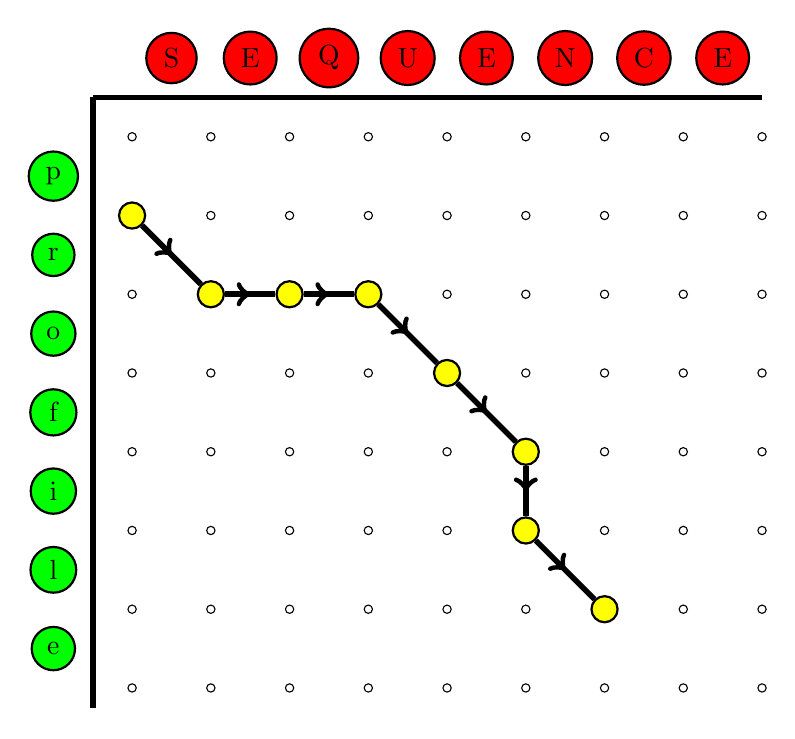
\begin{tikzpicture}
	\begin{pgfonlayer}{nodelayer}
		\node [style=newstyle] (0) at (-9, 3.5) {};
		\node [style=newstyle] (1) at (-8, 3.5) {};
		\node [style=newstyle] (2) at (-7, 3.5) {};
		\node [style=newstyle] (3) at (-6, 3.5) {};
		\node [style=newstyle] (4) at (-5, 3.5) {};
		\node [style=newstyle] (5) at (-4, 3.5) {};
		\node [style=newstyle] (6) at (-3, 3.5) {};
		\node [style=newstyle] (7) at (-3, 2.5) {};
		\node [style=newstyle] (8) at (-7, 2.5) {};
		\node [style=newstyle] (9) at (-6, 2.5) {};
		\node [style=newstyle] (10) at (-4, 2.5) {};
		\node [style=newstyle] (11) at (-5, 2.5) {};
		\node [style=newstyle] (12) at (-4, 1.5) {};
		\node [style=newstyle] (13) at (-3, 1.5) {};
		\node [style=newstyle] (14) at (-9, 2.5) {};
		\node [style=newstyle] (15) at (-5, 1.5) {};
		\node [style=newstyle] (16) at (-4, 0.5) {};
		\node [style=newstyle] (17) at (-3, 0.5) {};
		\node [style=newstyle] (18) at (-9, 0.5) {};
		\node [style=newstyle] (19) at (-7, 1.5) {};
		\node [style=newstyle] (20) at (-8, 0.5) {};
		\node [style=newstyle] (21) at (-8, 2.5) {};
		\node [style=newstyle] (22) at (-3, -1.5) {};
		\node [style=newstyle] (23) at (-5, 0.5) {};
		\node [style=newstyle] (24) at (-6, 1.5) {};
		\node [style=newstyle] (25) at (-9, -1.5) {};
		\node [style=newstyle] (26) at (-8, -2.5) {};
		\node [style=newstyle] (27) at (-7, -0.5) {};
		\node [style=newstyle] (28) at (-8, -1.5) {};
		\node [style=newstyle] (29) at (-4, -2.5) {};
		\node [style=newstyle] (30) at (-10, -2.5) {};
		\node [style=newstyle] (31) at (-7, -2.5) {};
		\node [style=newstyle] (32) at (-10, -1.5) {};
		\node [style=newstyle] (33) at (-9, -2.5) {};
		\node [style=newstyle] (34) at (-5, -0.5) {};
		\node [style=newstyle] (35) at (-3, -2.5) {};
		\node [style=newstyle] (36) at (-8, -0.5) {};
		\node [style=newstyle] (37) at (-4, -1.5) {};
		\node [style=newstyle] (38) at (-10, -0.5) {};
		\node [style=newstyle] (39) at (-6, -2.5) {};
		\node [style=rn] (40) at (-10.5, 4.5) {S};
		\node [style=rn] (41) at (-9.5, 4.5) {E};
		\node [style=rn] (42) at (-8.5, 4.5) {Q};
		\node [style=rn] (43) at (-7.5, 4.5) {U};
		\node [style=rn] (44) at (-6.5, 4.5) {E};
		\node [style=rn] (45) at (-5.5, 4.5) {N};
		\node [style=rn] (46) at (-4.5, 4.5) {C};
		\node [style=rn] (47) at (-3.5, 4.5) {E};
		\node [style=gn] (48) at (-12, 3) {p};
		\node [style=gn] (49) at (-12, 2) {r};
		\node [style=gn] (50) at (-12, 1) {o};
		\node [style=gn] (51) at (-12, -0) {f};
		\node [style=gn] (52) at (-12, -1) {i};
		\node [style=gn] (53) at (-12, -2) {l};
		\node [style=gn] (54) at (-12, -3) {e};
		\node [style=yn] (55) at (-11, 2.5) {};
		\node [style=yn] (56) at (-10, 1.5) {};
		\node [style=yn] (57) at (-9, 1.5) {};
		\node [style=yn] (58) at (-8, 1.5) {};
		\node [style=yn] (59) at (-7, 0.5) {};
		\node [style=yn] (60) at (-6, -0.5) {};
		\node [style=yn] (61) at (-6, -1.5) {};
		\node [style=none] (62) at (-11.5, 4) {};
		\node [style=none] (63) at (-11.5, -3.75) {};
		\node [style=none] (64) at (-3, 4) {};
		\node [style=newstyle] (65) at (-5, -1.5) {};
		\node [style=newstyle] (66) at (-11, 0.5) {};
		\node [style=newstyle] (67) at (-10, 2.5) {};
		\node [style=newstyle] (68) at (-11, 1.5) {};
		\node [style=newstyle] (69) at (-11, 3.5) {};
		\node [style=newstyle] (70) at (-11, -1.5) {};
		\node [style=newstyle] (71) at (-11, -2.5) {};
		\node [style=newstyle] (72) at (-11, -0.5) {};
		\node [style=newstyle] (73) at (-7, -3.5) {};
		\node [style=newstyle] (74) at (-11, -3.5) {};
		\node [style=newstyle] (75) at (-8, -3.5) {};
		\node [style=newstyle] (76) at (-10, -3.5) {};
		\node [style=newstyle] (77) at (-6, -3.5) {};
		\node [style=newstyle] (78) at (-9, -3.5) {};
		\node [style=newstyle] (79) at (-4, -3.5) {};
		\node [style=newstyle] (80) at (-3, -3.5) {};
		\node [style=yn] (81) at (-5, -2.5) {};
		\node [style=newstyle] (82) at (-10, 3.5) {};
		\node [style=newstyle] (83) at (-10, 0.5) {};
		\node [style=newstyle] (84) at (-4, -0.5) {};
		\node [style=newstyle] (85) at (-3, -0.5) {};
		\node [style=newstyle] (86) at (-9, -0.5) {};
		\node [style=newstyle] (87) at (-5, -3.5) {};
		\node [style=newstyle] (88) at (-6, 0.5) {};
		\node [style=newstyle] (89) at (-7, -1.5) {};
	\end{pgfonlayer}
	\begin{pgfonlayer}{edgelayer}
		\draw [style=arrow] (55) to (56);
		\draw [style=arrow] (56) to (57);
		\draw [style=arrow] (57) to (58);
		\draw [style=arrow] (58) to (59);
		\draw [style=arrow] (59) to (60);
		\draw [style=arrow] (60) to (61);
		\draw [style=simple] (62.center) to (63.center);
		\draw [style=simple] (62.center) to (64.center);
		\draw [style=arrow] (61) to (81);
	\end{pgfonlayer}
\end{tikzpicture}
    \end{center}
  The capital letters represent sequence residues, the lower-case letters represent profile match positions.  Profile insert positions are not
  marked by symbols. They occur at the beginning, at the end, and between any pair of consecutive match positions of the profile.\\
  The path marked by horizontal, vertical, and diagonal bars defines the following alignment:
  \begin{center}
\begin{verbatim}
                 S E Q U E - N
                 r - - o f i l
\end{verbatim}
\end{center}
  Such an alignment can also be defined by a sequence of path matrix coordinates. By convention, the upper left corner of the matrix is assigned
  co-ordinates (0,0). Note that path matrix co-ordinates correspond to profile insert positions rather than match positions. Likewise, they fall
  between consecutive residues of the sequence. The above alignment is defined by the following coordinate sequence.
  \begin{equation*}
     (1,0) ,\, (2,1) ,\, (2,2) ,\, (2,3) ,\, (3,4) ,\, (4,5) ,\, (5,5) ,\, (6,6)
  \end{equation*}
  In general, a coordinate sequence $(i_0,j_0),\, (i_1,j_1) \ldots (i_L, j_L)$ defines a valid sequence alignment between a profile of length $N$
  and a sequence of length $M$ if and only if $i_k \in [0 ,\, N ]$, $j_k \in [0,\, M]$, $\forall k=0\ldots L$ and 
  \begin{equation*}
    \left \{ 
    \begin{array}{ccc}
     i_k + 1 = i_{k+1} &,& j_k + 1 = j_{k+1} \\
     i_k     = i_{k+1} &,& j_k + 1 = j_{k+1} \\
     i_k + 1 = i_{k+1} &,& j_k     = j_{k+1} 
     \end{array}
     \right.
  \end{equation*}
  $\forall k \in \left [0,\, L-1 \right ]$.   
     
  \begin{notes}
  \begin{itemize}
    \item The above definition encompasses both global and local types of alignments. In the following, it is not necessary to distinguish between
	  these two alternatives. A global alignment may simply be viewed as a limit case of a local alignment.
    \item The alignment definition underlying generalised profiles is equivalent
	  to the path definition of hidden Markon models in the following sense:
   \begin{enumerate}
      \item for a sequence and a profile of given lengths $M$, $N$, the number of possible alignments is exactly identical to the number of paths through
	    which an HMM of length $N$ can generate sequences of length $M$,
      \item there is an obvious one-to-one mapping between profile-sequence alignments and paths through HMMs; see also \cite{Bucher96}.
   \end{enumerate}
  \end{itemize}
  \end{notes}

  \subsection{Definition of the similarity score}

  The similarity score of a profile sequence-alignment is the sum of the scores assigned to its scorable components. The scorable components of an
  alignment are:
  \begin{it}
  \begin{enumerate}[i)]
  \item the beginning
  \item each extension step
  \item each state transition
  \item the end
  \end{enumerate}
  \end{it}
  Some of these terms need further explanation.

  An extension step occurs between any pair of consecutive path matrix coordinates. There are three different types of extension steps: \emph{match},
  \emph{insert}, and \emph{deletion} steps. In the above diagram, diagonal bars correspond to match extension steps, horizontal bars correspond to insert
  extension steps, and vertical bars correspond to deletion extension steps. The number of extension steps defines the length of the alignment.

  The type of an extension step is also called a state. Each extension step is thus associated with a match, insert, or deletion state. At the beginning, 
  an alignment is in \emph{initiation} state. At the end, it is in \emph{termination} state.  Initiation, match, insert, deletion, and termination
  states will be symbolised by the letters \textbf{B}, \textbf{M}, \textbf{I}, \textbf{D}, and \textbf{E} , respectively.

  A state transition occurs between any two consecutive alignment components associated with a state. Thus, there is one state transition for each coordinate
  pair of the alignment, including the first and the last. Note that this definition implies that state transitions also occur between identical states.\\
  In summary, an alignment of length $L$ has:\\
  \begin{center}
  \begin{tabular}{cl}
   $1$ & beginning \\
   $L$ & extensions steps \\
  $L+1$ & state transitions \\
   $1$ & termination \\
   \hline \\
  $2L+3$ & scorable components in total.
  \end{tabular}
  \end{center}
  
  All component scores are provided by the profile in a position-specific manner.  Therefore, the similarity score does not depend on any parameter
  of an alignment method. The types and functions of profile scores are now explained.

  The scores assigned to the beginning and end of the alignment are called \emph{initiation} and \emph{termination} scores. These scores are distinct from
  those assigned to the first and last state transition though they correspond to the same path matrix co-ordinates. There are two types of
  scores for each class. The \emph{external} initiation score applies to coordinates at the beginning of the sequence. The \emph{internal} initiation
  score applies to all other co-ordinates. External and internal termination scores are defined analogously. The function of these scores is to
  flexibly encode local or global alignment scoring modes.  In addition, they may serve to anchor a motif at the beginning or at the end of a sequence.

  The scores for extension steps comprise three classes: match extension scores, insert extension scores, and deletion extension scores. Match and
  insert extension scores are residue-specific because the corresponding alignment steps span one sequence residue. By contrast, there is only one
  deletion extension score per profile position because deletion steps do not involve sequence residues.

  There are 16 different types of state transition scores for all possible transitions from an element of \{ \textbf{B}, \textbf{M}, \textbf{I}, \textbf{D} \}
  to an element of \{ \textbf{M}, \textbf{I}, \textbf{D}, \textbf{E} \}. State transition scores serve similar functions as gap opening penalties in a
  sequence-sequence alignment.

  \subsection{Basic profile structure}

  The basic profile structure follows almost conclusively from the forgoing definitions of a profile-sequence alignment and its similarity score.
  What remains to be clarified are a few details.

  A profile is based on a particular alphabet. The alphabet is considered a basic constituent of the profile because it determines the exact number of
  parameters per insert and match position. \\
  The two standard character sets for biomolecular patterns are:
  \begin{center}
  \begin{tabular}{ll}
   $\{ A,C,G,T \} $ & for nucleic acid motifs. \\
   $\{A,B,C,D,E,F,G,H,I,K,L,M,N,P,Q,R,S,T,V,W,Y,Z\}$ & for protein motifs.
  \end{tabular}
  \end{center}

  Other alphabets, e.g. alphabets including ambiguous codes for nucleotides, may be useful in particular circumstances.

  There is one insert and one match extension score for each character of the alphabet.  In practice, it is useful to define one additional insert
  and match extension score to deal with unexpected characters appearing in real sequences.

  Some of the previously introduced profile scores are associated with insert positions, others with match positions. A look at the path matrix
  diagram makes clear which type of score is associated with which type of profile position.

  An insert position of a profile based on a $K$-letter alphabet contains the following parameters:
  \begin{center}
  \begin{tabular}{ll}
   $1$ & external initiation score\\
   $1$ & internal initiation score\\
   $16$ & state transition scores for all transitions between elements of \{ \textbf{B}, \textbf{M}, \textbf{I}, \textbf{D} \} and \{ \textbf{M}, \textbf{I}, \textbf{D}, \textbf{E} \} \\
   $K$ & insert extension scores for each character of the alphabet\\
   $1$ & insert extension score for an unexpected character\\
   $1$ & internal termination score\\
   $1$ & external termination score\\
  \hline\\
  $K+21$ & insert position scores in total
  \end{tabular}
  \end{center}
  
  A match position of a profile based on a K-letter alphabet contains the following parameters.
  \begin{center}
  \begin{tabular}{ll}
   $K$ & match extension scores for each letter of the alphabet\\
   $1$ & match extension score for an unexpected character\\
   $1$ & deletion extension score\\
  \hline \\
  $K+2$ & match position scores in total
  \end{tabular}
  \end{center}
  
  Admissible values for profile scores are any integer or real number plus a special value representing a forbidden alignment step. This value will be
  called \emph{low-value} and behaves like minus infinity in mathematical operations.

  A profile has also a defined topology, either linear or circular.  Most profiles will be linear.  Circular profiles may represent motifs which
  consist of a variable number of tandemly repeated units.  Note that a linear profile begins and ends with an insert position.

  \begin{notes}
 \begin{itemize}
  \item The above list of position-specific profile scores represents the maximum number of supported features. Real profiles derived with an 
  existing method will rarely use all of them. Concise representation of a profile can be achieved through specification of appropriate defaults;
   see examples in Section \ref{Examples}.
  \item There is some redundancy in the implemented parameter set allowing for alternative representations of functionally equivalent profiles. This
   freedom could be used for scaling profile scores in units related to a particular mathematical or physical interpretation, e.g. probabilities
   of a hidden Markov model or thermodynamic quantities.
  \item The above definition of a sequence alignment assumes linear topology
   for both the profile and the sequence. Generalisation to circular topology is straightforward. An alignment between a circular profile and
   a linear sequence, or between a linear profile and a circular sequence, corresponds to a path on a cylindrical surface. An alignment between a
   circular profile and a circular sequence corresponds to a path on a torus.
 \end{itemize}
 \end{notes}

 \section{Profile accessories} \label{Profile accessories}
 
  The primary purpose of a profile is to identify as reliably as possible biologically relevant motif occurrences in new sequences. 
  The basic profile structure described in the previous Section is not sufficient to define a rational search strategy to this end. The accessory profile
  features presented here fill this gap. Appropriately interpreted, they complement the position-specific profile scores to provide determinative
  instruction for a motif search. In addition, they guide the interpration of potential matches.

  \subsection{Cut-off value}

  For a profile and a sequence of typical lengths, there is a very large number of possible alignments. At most a few of them will be biologically
  relevant. The function of a cut-off value is to a priori exclude a large number of alignments from further consideration by a profile search algorithm.
  The fate of the remaining alignments with similarity scores greater than or equal to the cut-off value depends on a specific disjointness definition
  applied; see below.

  An important aspect of a cut-off value is that it gives a qualitative meaning to a profile. This is a prerequisite for statistics on false positives
  and false negatives obtained in a database search, as currently provided by PROSITE.

  In certain situations, it is useful to supply more than one cut-off value, partitioning the range of alignment scores into multiple areas. The areas
  may correspond to different degrees of certainty, ranges of evolutionary distance, or levels of physiological activity.


  \subsection{Score normalisation instructions}

  The profile-alignment scores defined in the previous Section are called raw scores. In most cases, they will not lend themselves to meaningful
  biological interpretations and will therefore not be very helpful in the interpretation of a potential match. In practice, one is interested in
  questions like: What is the probability of finding a match of a certain score in a random sequence? How does the similarity score relate to a
  measurable property of the biological object? The purpose of normalisation instructions is to convert the raw score into directly interpretable units.

  There may be multiple normalisation modes for the same profile, each one associated with a different mathematical, physical, or biological interpretation;
  see examples in Section \ref{Examples}.

  Normalisation functions are required to preserve the ranking of scores pertaining to alternative alignments between the same profile and the same
  sequence. However, since normalisation functions may depend on sequence parameters such as length and residue composition, they will generally not
  preserve the order of scores pertaining to matches from different sequences arising in a database search.

  \begin{notes}
  \begin{itemize}
  \item Cut-off values may be defined in raw score units or normalised score units.
  \item Programs may rely on normalised rather than raw scores for various operation, e.g. sorting of accepted matches in a database search.
  \item An expanding list of normalisation functions is presented in Appendix \ref{Normalization functions}.
  \end{itemize}
  \end{notes}


  \subsection{Disjointness definitions}

  There are situations where only a single best alignment and its similarity score are of interest. This arises for instance with a profile serving
  exclusively as a signature for a protein family.  More frequently, the same motif may occur more than once in a given sequence, and each occurrence will be of interest.

  In the first case, the motif search problem is simple and can be solved by a standard optimal alignment algorithm such as described in \cite{Gribskov90}. In the
  second case, the task is more difficult and needs to be explained in more detail.

  At first glance, the problem seems to be to find all profile-sequence alignments with similarity scores greater than or equal to the cut-off
  value. However, such an approach would not yield useful results because a high scoring alignment typically belongs to a large group of very similar
  alignments with comparable scores. Two members of such a group may differ only by an additional extension step at one end of one alignment. In
  sequence-sequence comparisons, a cluster of related  alignments  is represented by a single highest scoring member. This seems a reasonable
  procedure for profiles too.

  As a second approximation, one could therefore define the task of finding multiple profile matches in the same sequence as one of finding as many as
  possible, locally optimal, but mutually disjoint alignments with scores greater than or equal to the cut-off value. What is still missing in such
  a statement of the problem is a precise definition of disjointness and a tie-braking rule to choose between equally high-scoring alignments. The
  former is of fundamental importance and needs to be addressed here.  The latter may be considered a property of a specific algorithm and thus is
  beyond the scope of this document.

  There are many possible ways to define disjointness of two alignments. The algorithms described for finding multiple locally optimal alignments
  between pairs of sequences consider two alignments disjoint if they have no extension step in common \cite{Waterman87, Huang91}. The two alignments specified in the
  path matrix diagram below illustrate this notion of disjointness.
  \begin{center}
  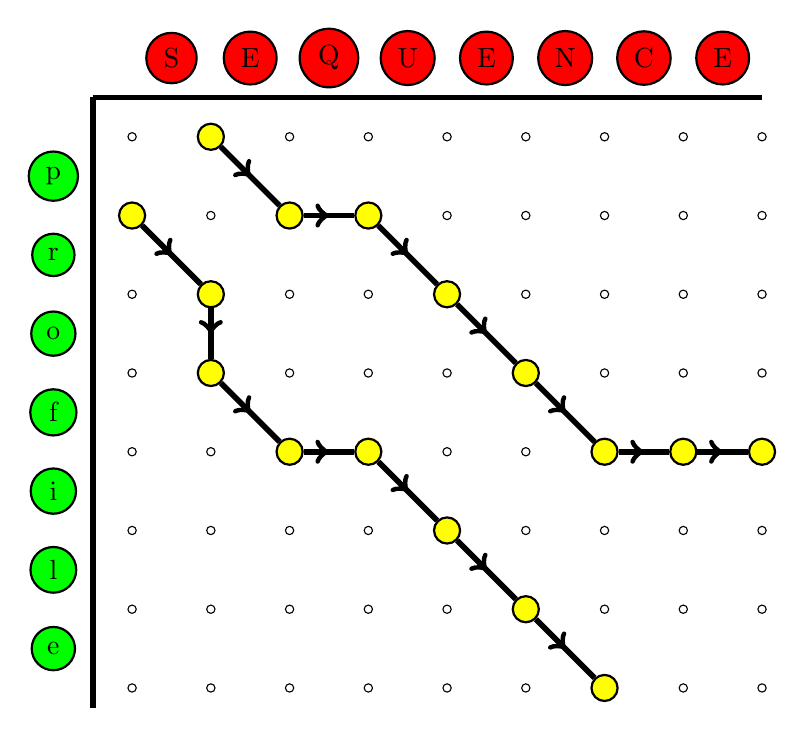
\begin{tikzpicture}
	\begin{pgfonlayer}{nodelayer}
		\node [style=newstyle] (0) at (-9, 3.5) {};
		\node [style=newstyle] (1) at (-8, 3.5) {};
		\node [style=newstyle] (2) at (-7, 3.5) {};
		\node [style=newstyle] (3) at (-6, 3.5) {};
		\node [style=newstyle] (4) at (-5, 3.5) {};
		\node [style=newstyle] (5) at (-4, 3.5) {};
		\node [style=newstyle] (6) at (-3, 3.5) {};
		\node [style=newstyle] (7) at (-3, 2.5) {};
		\node [style=newstyle] (8) at (-7, 2.5) {};
		\node [style=newstyle] (9) at (-6, 2.5) {};
		\node [style=newstyle] (10) at (-4, 2.5) {};
		\node [style=newstyle] (11) at (-5, 2.5) {};
		\node [style=newstyle] (12) at (-4, 1.5) {};
		\node [style=newstyle] (13) at (-3, 1.5) {};
		\node [style=newstyle] (14) at (-9, 1.5) {};
		\node [style=newstyle] (15) at (-5, 1.5) {};
		\node [style=newstyle] (16) at (-4, 0.5) {};
		\node [style=newstyle] (17) at (-3, 0.5) {};
		\node [style=newstyle] (18) at (-9, 0.5) {};
		\node [style=newstyle] (19) at (-7, 0.5) {};
		\node [style=newstyle] (20) at (-8, 0.5) {};
		\node [style=newstyle] (21) at (-8, 1.5) {};
		\node [style=newstyle] (22) at (-3, -1.5) {};
		\node [style=newstyle] (23) at (-5, 0.5) {};
		\node [style=newstyle] (24) at (-6, 1.5) {};
		\node [style=newstyle] (25) at (-9, -1.5) {};
		\node [style=newstyle] (26) at (-8, -2.5) {};
		\node [style=newstyle] (27) at (-7, -0.5) {};
		\node [style=newstyle] (28) at (-8, -1.5) {};
		\node [style=newstyle] (29) at (-4, -2.5) {};
		\node [style=newstyle] (30) at (-10, -2.5) {};
		\node [style=newstyle] (31) at (-7, -2.5) {};
		\node [style=newstyle] (32) at (-10, -1.5) {};
		\node [style=newstyle] (33) at (-9, -2.5) {};
		\node [style=newstyle] (34) at (-6, -1.5) {};
		\node [style=newstyle] (35) at (-3, -2.5) {};
		\node [style=newstyle] (36) at (-6, -0.5) {};
		\node [style=newstyle] (37) at (-4, -1.5) {};
		\node [style=newstyle] (38) at (-10, -0.5) {};
		\node [style=newstyle] (39) at (-5, -2.5) {};
		\node [style=rn] (40) at (-10.5, 4.5) {S};
		\node [style=rn] (41) at (-9.5, 4.5) {E};
		\node [style=rn] (42) at (-8.5, 4.5) {Q};
		\node [style=rn] (43) at (-7.5, 4.5) {U};
		\node [style=rn] (44) at (-6.5, 4.5) {E};
		\node [style=rn] (45) at (-5.5, 4.5) {N};
		\node [style=rn] (46) at (-4.5, 4.5) {C};
		\node [style=rn] (47) at (-3.5, 4.5) {E};
		\node [style=gn] (48) at (-12, 3) {p};
		\node [style=gn] (49) at (-12, 2) {r};
		\node [style=gn] (50) at (-12, 1) {o};
		\node [style=gn] (51) at (-12, -0) {f};
		\node [style=gn] (52) at (-12, -1) {i};
		\node [style=gn] (53) at (-12, -2) {l};
		\node [style=gn] (54) at (-12, -3) {e};
		\node [style=yn] (55) at (-11, 2.5) {};
		\node [style=yn] (56) at (-10, 1.5) {};
		\node [style=yn] (57) at (-10, 0.5) {};
		\node [style=yn] (58) at (-9, -0.5) {};
		\node [style=yn] (59) at (-8, -0.5) {};
		\node [style=yn] (60) at (-7, -1.5) {};
		\node [style=yn] (61) at (-6, -2.5) {};
		\node [style=none] (62) at (-11.5, 4) {};
		\node [style=none] (63) at (-11.5, -3.75) {};
		\node [style=none] (64) at (-3, 4) {};
		\node [style=newstyle] (65) at (-5, -1.5) {};
		\node [style=yn] (66) at (-10, 3.5) {};
		\node [style=yn] (67) at (-9, 2.5) {};
		\node [style=yn] (68) at (-8, 2.5) {};
		\node [style=yn] (69) at (-7, 1.5) {};
		\node [style=yn] (70) at (-6, 0.5) {};
		\node [style=yn] (71) at (-5, -0.5) {};
		\node [style=yn] (72) at (-4, -0.5) {};
		\node [style=newstyle] (73) at (-11, 0.5) {};
		\node [style=newstyle] (74) at (-10, 2.5) {};
		\node [style=newstyle] (75) at (-11, 1.5) {};
		\node [style=newstyle] (76) at (-11, 3.5) {};
		\node [style=newstyle] (77) at (-11, -1.5) {};
		\node [style=newstyle] (78) at (-11, -2.5) {};
		\node [style=newstyle] (79) at (-11, -0.5) {};
		\node [style=newstyle] (80) at (-7, -3.5) {};
		\node [style=newstyle] (81) at (-11, -3.5) {};
		\node [style=newstyle] (82) at (-8, -3.5) {};
		\node [style=newstyle] (83) at (-10, -3.5) {};
		\node [style=newstyle] (84) at (-6, -3.5) {};
		\node [style=newstyle] (85) at (-9, -3.5) {};
		\node [style=newstyle] (86) at (-4, -3.5) {};
		\node [style=newstyle] (87) at (-3, -3.5) {};
		\node [style=yn] (88) at (-5, -3.5) {};
		\node [style=yn] (89) at (-3, -0.5) {};
	\end{pgfonlayer}
	\begin{pgfonlayer}{edgelayer}
		\draw [style=arrow] (55) to (56);
		\draw [style=arrow] (56) to (57);
		\draw [style=arrow] (57) to (58);
		\draw [style=arrow] (58) to (59);
		\draw [style=arrow] (59) to (60);
		\draw [style=arrow] (60) to (61);
		\draw [style=simple] (62.center) to (63.center);
		\draw [style=simple] (62.center) to (64.center);
		\draw [style=arrow] (66) to (67);
		\draw [style=arrow] (67) to (68);
		\draw [style=arrow] (68) to (69);
		\draw [style=arrow] (69) to (70);
		\draw [style=arrow] (70) to (71);
		\draw [style=arrow] (71) to (72);
		\draw [style=arrow] (61) to (88);
		\draw [style=arrow] (72) to (89);
	\end{pgfonlayer}
  \end{tikzpicture}
  \end{center}

  However, such a definition will not be adequate for many motif search application because it allows the same sequence residue to be matched with
  different profile positions. Imagine the case of a protein structural domain.  There, it is inconceivable that the same residue simultaneously
  participates in the formation of two physically distinct domains, occupying different places within these domains.

  There may be no single disjointness definition adequate for all kinds of biological sequence motifs which can be characterised by a profile. For
  this and other reasons, a specific notion of disjointness is viewed and implemented as a profile-inherent property rather than a variable of the
  alignment method. In some cases, a particular definition may even be derived from a measurable property of the biological object.
  The concluding example illustrates this point.

  The DNA recognition site of mammalian transcription factor Sp1 is about $14$ bp long and can be fairly accurately represented by a conventional weight
  matrix. Experiments have shown that the minimal center-to-center distance for two sites to be simultaneously occupied by two proteins is 10 bp. For
  a profile representing an Sp1 binding site, an appropriate criterion for disjointness would require that the sequence segments aligned with the
  central 10 bp region of the recognition motif do not overlap.

  \begin{notes}
  \begin{itemize}
  \item The problems related to disjoint alignments are not specific to profiles. They also occur with qualitative variable-length patterns based
   on a regular expression-like syntax.
  \item An expanding list of alternative disjointness definitions is presented in Appendix \ref{Disjointness definitions}.
  \item The algorithms for multiple pairwise sequence alignments described in \cite{Waterman87, Huang91} can easily be adjusted to the disjointness definitions proposed
   in Appendix \ref{Disjointness definitions}.
  \item Another principle for parsing multiple matches between an HMM and a sequence is implemented in the HMMER programs hmmls and hmmfs \cite{Eddy96}.
  \end{itemize}
  \end{notes}

  \section{A machine-readable text file format} \label{A machine-readable text file format}
  
  This Section describes the format conventions used in the PROSITE data bank for representation of profiles


  \subsection{General format of the MA line}
  The current PROSITE database reserves the MA line code for information specific to matrix entries.

  A profile typically extends over many MA lines. The general format of a block of consecutive MA lines is as follows:
\begin{verbatim}
  MA  /KEYWORD: parameter=value; parameter=value; ... ; /KEYWORD:
  MA  parameter=value; parameter=value; ... ; /KEYWORD: ...
\end{verbatim}
  The text is substructured into so-called data blocks, each one beginning with a keyword followed by a list of parameter specifications. Keywords
  identify different types of data blocks with characteristic parameter subsets. The keywords at the beginning of each data block are enclosed by
  slash on the left side and by colon on the right side. Individual parameter specifications are delimited by semicolon. There is also a semicolon
  at the end of each data block containing at least one parameter specification.

  A single word, quoted string, or number must be contained within one line. Otherwise, there are no rules guiding the placement of text units onto
  physical lines. Within one block, the parameter specifications can appear in any order.

  The following keywords define valid data block types:
  \begin{center}
  \begin{tabular}{rl}
    /GENERAL\_SPEC: &   General specifications.\\
    /DISJOINT:      &   Disjointness definition for multiple matches.\\
    /NORMALIZATION: &   Score normalisation instructions.\\
    /CUT\_OFF:      &   Recommended cut-off value(s).\\
    /DEFAULT:       &   Defaults for position specific profile parameters.\\
    /I:             &   Profile insert position.\\
    /M:             &   Profile match position.
  \end{tabular}
  \end{center}

  \subsection{The formats of different data block types}

  \subsubsection{The GENERAL\_SPEC data block}

  The GENERAL\_SPEC data block provides general information about the profile. It has the following format:
\begin{verbatim}
  /GENERAL_SPEC: ALPHABET=string;
                 [ LENGTH=length; TOPOLOGY=topology; BEGIN=begin; END=end ]
                 [ LOG\_BASE=log\_base; P0=p0; P=random\_model ]
\end{verbatim}
  where:
  \begin{description}
  \item[string] is a quoted character string defining the character set for which, and the order in which, position-specific match and insert
      extension scores are provided in subsequent M and I data blocks.
  \item[length] is the length of the profile defined as the total number of match positions.
  \item[topology] is one of the alternative words LINEAR or CIRCULAR.
  \item[begin] is an integer indicating the match position withing the profile where the described biological object begins (implying that positions
      before \emph{begin} characterise contextual constraints). This together with the END feature may be useful for profiles characterising biological objects
      such as transmembrane helices in proteins, or exons in gene sequences.  As an instruction to software, this parameter means that sequence residues matching
      profile positions before the \emph{begin} position should not be reported as being part of the biological object.
  \item[end] is an integer indicating the match position within the profile where the biological object ends; see also remarks on previous parameter.
  \item[log\_base] is the logarithmic base that should be used when translating the generalised profile (back) into an HMM, see \cite{Bucher96}. Popular logarithmic
      bases for the representation of HMMs, null-models, substitution matrices, etc. are tabulated in Appendix \ref{Frequently used logarithmic bases}.
  \item[p0] is a real number between $0$ and $1$ defining the insert-to-insert state transition probability of the null-model that should be used for
      translating the generalised profile (back) into an HMM; see \cite{Bucher96}. This parameter defines a geometric length distribution over the sequence space.
  \item[random-model] is a real number, or comma separated list of real numbers, defining the residue emission probabilities of the null-model
      that should be used for translating the generalised profile (back) into an HMM; see \cite{Bucher96}. These numbers are not required to sum to $1$ and thus
      should be renormalised by programs on input. In PROSITE, the random model is usually given as percent amino acid frequencies.
 \end{description}
  
  The GENERAL\_SPEC data block is mandatory and precedes any DEFAULT, M or I data block.

  Implicit defaults:
  \begin{itemize}
  \item TOPOLOGY=LINEAR;
  \end{itemize}
  Example:

  MA  /GENERAL\_SPEC: ALPHABET='ACGT';

  \begin{notes}
   The optional LENGTH parameter is purely informative and redundant. The actual length of the profile is given by the sequence of subsequent I
   and M data blocks.
  \end{notes}
  
  

  \subsubsection{The DISJOINT data block}

  The DISJOINT data block provides a definition of disjointness for multiple profile-sequence alignments, or indicates that only one globally optimal
  alignment is of interest. It has the following format:
\begin{verbatim}
  /DISJOINT: DEFINITION=name; parameters;
\end{verbatim}
  where:
  \begin{description}
  \item[name] is a word from a controlled vocabulary identifying one of the supported disjoint definitions listed in Appendix \ref{Disjointness definitions}.
  \item[parameters] is a list of parameter specifications for the corresponding disjointness definition. Note that different disjointness 
    definitions depend on different parameter sets; see Appendix \ref{Disjointness definitions}.
  \end{description}
    
  The DISJOINT data block is mandatory.

  Example:

  MA  /DISJOINT: DEFINITION=PROTECT; N1=12; N2=40;

  \begin{notes}
  \begin{itemize}
  \item Some disjointness definitions are parameter-free. In this case, the list of parameter specifications is empty.
  \item The list of supported disjoint definitions constitutes a dynamic feature of the format.  New functions may be added in the future.
   Suggestions are welcome.
 \end{itemize}
 \end{notes}

 \subsubsection{The NORMALIZATION data block}

  A NORMALIZATION data block describes a specific normalisation mode for alignment scores. It has the following format:
\begin{verbatim}
  /NORMALIZATION: FUNCTION=name; parameters;
                  [ MODE=mode-nr; PRIORITY=rank; TEXT=string; ]
\end{verbatim}
  where:
  \begin{description}
    \item[name] is a word form a controlled vocabulary identifying one of the supported normalisation functions listed in Appendix \ref{Normalization functions}.
    \item[parameters] is a list of parameter specifications providing values for all parameters of the corresponding normalisation function listed in
    Appendix \ref{Normalization functions}.
    \item[mode-nr] is an integer by which the normalisation mode can be referred to in CUT\_OFF data blocks.
    \item[rank] is an integer assigning a relative priority to the normalisation mode with regard to various pattern search operations.
    \item[string] is a quoted string describing a score normalised according to this mode.
  \end{description}
  
  NORMALIZATION data blocks are optional. There may be several NORMALIZATION data blocks per profile.

  The optional MODE parameter either appears in all or in none of the NORMALIZATION data blocks. If specified, the mode numbers form a contiguous
  integer range starting with 1. If not specified, mode numbers are implied by the order in which the NORMALIZATION data blocks appear in the profile.

  The optional PRIORITY parameter either appears in all or none of the NORMALIZATION data blocks. If not specified, priorities are equal to the mode
  numbers. The lower the priority number, the higher the priority of the normalisation mode, and vice-versa.

  Example:

  MA  /NORMALIZATION: MODE=1; FUNCTION=LINEAR; TEXT='Homology Score';
  MA   R1=-90.558; R2=0.57225;

  \begin{notes}
  \begin{itemize}
  \item Normalisation functions may, in addition to the parameters listed in Appendix\ref{Normalization functions}, depend on characteristics of the sequence such as length
   and residue composition.
 \end{itemize}
 \end{notes}

 \subsubsection{The CUT\_OFF data block}

  A CUT\_OFF data block defines a cut-off level. It has the following format:
\begin{verbatim}
  /CUT_OFF: SCORE=rscore;
             [ LEVEL=level; TEXT=string; N\_SCORE=nscore; MODE=mode-nr ]
\end{verbatim}
  where:
  \begin{description}
  \item[rscore] is an integer defining the cut-off value in raw score units.
  \item[level] is an integer identifying a cut-off level.
  \item[string] is a quoted character string characterising profile matches with scores greater than or equal to the corresponding cut-off value
	(but lower than any higher cut-off value specified).
  \item[nscore] is a real number, or a comma separated list of real numbers, defining the cut-off value(s) in normalised score units calculated 
	according to the mode(s) identified by mode-nr.
  \item[mode-nr] is an integer, or a comma separated list of integers, referring to one or several normalisation modes defined in NORMALIZATION
   data blocks.
  \end{description}
  
  The CUT\_OFF data block for level 0 is mandatory. There may be multiple CUT\_OFF data blocks, one for each level.

  The LEVEL parameter is optional for level 0. All other levels are specified explicitly.  The levels assigned to alternative cut-off values, including
  level $0$, form a contiguous integer range.

  The N\_SCORE and MODE parameters are either both present or both absent. If present, they contain the same number of elements.

  Example:

  MA  /CUT\_OFF: LEVEL=0; SCORE=237; N\_SCORE=7.5; MODE=1;

  \begin{notes}
  \begin{itemize}
  \item Cut-off values in raw score units may be used by programs which do not support a given normalisation mode.
  \item The list of supported normalisation functions constitutes a dynamic feature of the format.  New functions may be added in the future.
   Suggestions are welcome.
 \end{itemize}
 \end{notes}

 \subsubsection{The DEFAULT data block}

  The DEFAULT data block redefines defaults for position-specific profile parameters and has the following format:
\begin{verbatim}
  /DEFAULT: [ SY_I=char1; SY_M=char2; parameters; ]
\end{verbatim}
  where:
  \begin{description}
  \item[char1] is a quoted character representing a profile insert position in a profile-sequence alignment.
  \item[char2] is a quoted character representing a profile match position in a profile-sequence alignment.
  \item[parameters] is a list of parameter specifications defining default values for one or several of the profile scores listed in the tables at
	the end of this Section.
  \end{description}
  
  DEFAULT data blocks are optional. There may be multiple DEFAULT data
  blocks per profile.

  Implicit defaults:

  - SY\_I='-'; SY\_M='X';

  Example:

  MA  /DEFAULT: B0= *; B1= *; E0= *; E1= *;

  \begin{notes}
  \begin{itemize}
  \item The first DEFAULT data block redefines the implicit defaults given in the tables at the end of this Section. Subsequent DEFAULT data blocks
   consecutively redefine each other.
  \item Asterisk represents low-value in the example; see next Subsection.
  \end{itemize}
  \end{notes}
  

  \subsubsection{The I and M data blocks}

  The I and M data blocks contain position-specific profile scores for insert and match positions. They have the following formats:
\begin{verbatim}
  /I: [ SY=char1; parameters; ]
  /M: [ SY=char2; parameters; ]
\end{verbatim}
  where:
  \begin{description}
  \item[char1] is a quoted character representing the corresponding profile insert position in a profile-sequence alignment.
  \item[char2] is a quoted character representing the corresponding profile match position in a profile-sequence alignment.
  \item[parameters] is a list of parameter specifications assigning values to one or several of the position-specific profile scores listed in the
   tables at the end of this Section.
  \end{description}
  
  The profile scores specified in I and M data blocks overwrite the current default values set by a preceding DEFAULT data block or initialised as
  shown in the tables at the end of this Section.

  The values assigned to profile scores may be integers, reals, or low-value represented by an asterisk. Most profile scores are assigned one value.
  The exceptions are the residue-specific insert and match extension scores. These scores can either be assigned one value or a comma separated list of
  values, one for each character of the alphabet. The correspondence between scores and characters is defined by the order in which the alphabet is
  presented in the GENERAL\_SPEC data block. A single value is equivalent to a list of identical values.

  Each I data block characterises one insert position of the profile.  Each M data block characterises one match position of the profile. The physical order 
  of the M and I data blocks defines the logical order of the corresponding profile positions. Default match and insert positions are
  not always specified explicitly.  This requires further explanation. Remember that a profile consists of an alternating sequence of insert and
  match positions, and that a linear profile starts and ends with an insert position.  Default I or M data block are implied wherever the physical
  order of I and M data blocks does not conform to these rules.

  Example:
\begin{verbatim}
  MA  /I: B0= 0; B1= 0; /M: M= 11, 3, 3, 4;
\end{verbatim}
  In case the above line describes a complete linear profile, a default insert position is implied at the end. In case it describes a circular profile, 
  no additional profile position is implied.

  \begin{notes}
  \begin{itemize}
  \item There has been some debate (and no decision so far) whether profile scores should be required to be integers. In PROSITE, all profile scores are represented
        as integers and existing software supporting this format actually requires integer representation. Integer representation has thus become a \emph{de facto} standard.
  \item A linear normalisation function implicitly defines an integer to real conversion of profile scores; see protein example in Section \ref{Examples}.
  \end{itemize}
  \end{notes}
  
  Profile scores of insert positions and implicit defaults:
  \begin{center}
  \begin{tabular}{rcl}
  Name & Default & Parameter description \\
  \hline \\
  B0  &B0= 0  &External initiation score\\
  B1  &B1= 0  &Internal initiation score\\
  E0  &E0= 0  &External termination score\\
  E1  &E1= 0  &Internal termination score\\
  \\
  BM  &BM= 0  &State transition score from state B to M\\
  BI  &BI= *  &State transition score form state B to I\\
  BD  &BD= *  &State transition score from state B to D\\
  BE  &BE= *  &State transition score from state B to E\\
  MM  &MM= 0  &State transition score from state M to M\\
  MI  &MI= *  &State transition score from state M to I\\
  MD  &MD= *  &State transition score from state M to D\\
  ME  &ME= 0  &State transition score from state M to E\\
  IM  &IM= *  &State transition score from state I to M\\
  II  &II= 0  &State transition score from state I to I\\
  ID  &ID= *  &State transition score from state I to D\\
  IE  &IE= *  &State transition score from state I to E\\
  DM  &DM= *  &State transition score from state D to M\\
  DI  &DI= *  &State transition score from state D to I\\
  DD  &DD= 0  &State transition score from state D to D\\
  DE  &DE= *  &State transition score from state D to E\\
  \\
  I   &I = 0  &Insert extension score(s) for characters included in the alphabet\\
  I0  &I0= 0  &Insert extension score for a character not included in the alphabet\\
  \hline
  \end{tabular}
  \end{center}
  
  Profile parameters of match positions and implicit defaults:
  \begin{center}
  \begin{tabular}{rcl}
  Name & Default & Parameter description \\
  \hline \\
  M   &M = 0  &Match extension score(s) for characters included in the alphabet\\
  M0  &M0= 0  &Match extension score for a character not included in the alphabet\\
  D   &D = 0  &Deletion extension score\\
  \hline
  \end{tabular}
  \end{center}
  
  \section{Examples} \label{Examples}

  \subsection{E. coli promoters}

  The profile shown below describes the major class of E. coli promoters
  recognised by RNA polymerase-sigma factor 70. It is based on work published in \cite{Mulligan84} and emulates the functionality of the promoter search program TARGSEARCH.

  \begin{verbatim}
MA  /GENERAL_SPEC: ALPHABET='ACGT';
MA  /DISJOINT: DEFINITION=PROTECT; N1=37; N2=42;
MA  /NORMALIZATION: MODE=1; FUNCTION=LINEAR; R1=-90.558; R2=0.57225;
MA   TEXT='Homology Score';
MA  /NORMALIZATION: MODE=2; FUNCTION=LINEAR; R1=-10.198; R2=0.06215;
MA   TEXT='Log KBk2';
MA  /CUT_OFF: LEVEL=0; SCORE=237; N_SCORE=45.0; MODE=1;
MA  /DEFAULT: B0=*; B1=*; E0=*; E1=*;
MA  /I: B0= 0; B1= 0;
MA  /M: M= 11, 3, 3, 4;
MA  /M: M= 8, 4, 2, 7;
MA  /M: M= 8, 2, 4, 7;
MA  /M: M= 7, 4, 2, 8;
MA  /M: M= 8, 4, 4, 5;
MA  /M: M= 7, 3, 5, 6;
MA  /M: M= 3, 5, 5, 8;
MA  /M: M= 5, 2, 5, 9;
MA  /M: M= 5, 8, 5, 3;
MA  /M: M= 0, 1, 2,17; SY='T';
MA  /M: M= 1, 1, 1,18; SY='T';
MA  /M: M= 0, 2,17, 2; SY='G';
MA  /M: M= 14, 3, 1, 4; SY='A';
MA  /M: M= 5,11, 2, 5; SY='C';
MA  /M: M= 9, 2, 3, 7; SY='A';
MA  /M: M= 5, 5, 3, 9;
MA   /M:/M:/M:/M:/M:/M:/M:/M:/M:
MA   /I: MD=0; MM=1;/I: DM=1;/I: DM=1;/I: DM=6;/I: DM=14;/I: DM=6;/I: DM=1;
MA  /M: M= 4, 5, 2,10;
MA  /M: M= 5, 4, 5, 6;
MA  /M: M= 3, 5, 5, 8;
MA  /M: M= 4, 4, 8, 5;
MA  /M: M= 4, 5, 7, 6;
MA  /M: M= 0, 2, 2,17; SY='T';
MA  /M: M= 20, 0, 0, 1; SY='A';
MA  /M: M= 5, 3, 3, 9; SY='T';
MA  /M: M= 12, 3, 3, 3; SY='A';
MA  /M: M= 11, 4, 3, 4; SY='A';
MA  /M: M= 0, 1, 0,20; SY='T';
MA  /M: M= 7, 2, 6, 6;
MA  /M: M= 4, 7, 5, 5;
MA  /M: M= 6, 6, 6, 4;
MA  /I: E0=0; E1= 0;
\end{verbatim}

  The profile is substructured into four operationally distinct modules totaling 45 match positions.
  \begin{center}
  \begin{tabular}{cp{15cm}}
  Position & Module \\
  \hline \\
   1-16  & Weight matrix for the -35 region including the core hexamer box TTGACA at pos. 10-15.\\
  17-25  & Fixed length linker module encoded by 9 dummy match positions. This module is defined on the first of the two indented MA lines.\\
  26-31  & Variable length linker scoring module encoded by 7 consecutive insert positions.  This module is defined on the second of two
           indented MA lines. \\
  32 -45 &  Weight matrix for the -10 region including the core hexamer box TATAAT at pos. 37-42.\\
  \hline \\
  \end{tabular}
  \end{center}
  The variable length linker scoring module defines the following scoring
  scheme.
  \begin{center}
  \begin{tabular}{cc}
    \# of bp between core  hexamers boxes & score \\
    \hline \\         
    $15$ & $1$\\
    $16$ & $6$\\
    $17$ & $14$\\
    $18$ & $6$\\
    $19$ & $1$\\
    $20$ & $1$\\
    $21$ & $1$
  \end{tabular}
  \end{center}

  These scores are achieved as follows. Format-proprietary default values for state transition scores (not over-written by local defaults) make sure
  that deletions and insertions can only occur at  positions  where corresponding scores are explicitly specified. Insertion gaps are thus
  generally forbidden. A deletion gap can only be opened at the beginning of the linker length scoring module and must be closed within or at the
  end of this module. A promoter with the maximal linker length of 21 can be aligned without gap to the profile. In this case, the linker length score
  is provided by MM=1 at insert position 25. Promoters with linker lengths 15 to 20 require a deletion gap in their alignment to the profile. The
  corresponding scores are provided by DM=1, 1, 6, 14, 6, 1 at insert positions 26, 27, 28, 29, 30, 31, respectively.

  \begin{notes}
  \begin{itemize}
  \item The default low-values assigned to parameters B0, B1, E0, E1, together
   with the exceptions B0, B1 = 0 at the beginning and E0, E1 = 0 at the
   end of the profile, define a global alignment algorithm with endgap
   weighting in the profile but not in the sequence.
  \item Two normalisation modes are defined in this profile. The names of the
   corresponding scores, \emph{Homology score} and \emph{log KBk2}, are taken from
   the original publication. The parameters of the second normalisation
   function were derived by a linear regression analysis between homology
   scores and enzyme selectivities (defined as log KBk2) of 31 transcriptionally assayed promoters.
  \item The cut-off homology score of 45 has been proposed by the authors as
   lower limit for effective promoters.
  \item The disjointness definition protecting only the TATAAT box region from
   sequence overlap, is motivated by a known promoter example where two
   adjacent TATAAT boxes direct transcription from two distinct initiation
   sites six bp apart from each other.
  \item This profile is not supposed to represent the most accurate E. coli
   promoter prediction method available today. It primarily serves to illustrate that the proposed syntax is flexible enough to express the
   functionality of a specialised search algorithm developed for a particular object.
 \end{itemize}
 \end{notes}

  \subsection{Src homology domain SH3}

  The profile shown on the next page describes the Src homology domain SH3
  as defined by sequence similarity. It has been constructed by a recently
  described extension of Gribskov's method incorporating several improvements \cite{Luethy94}.

  The SH3 profile consists of three homology blocks separated by two gap regions. Within the homology blocks, small insertions and deletions are not
  totally forbidden but strongly impeded by high gap costs defined in the
  DEFAULT data block: MI=-26, I=-3, MD=-26, D=-3. These numbers are overwritten by more permissive values in the two gap regions.

  \begin{notes}
  \begin{itemize}
  \item The SH3 profile uses only features which are compatible with Gribskov's
   methodology. As a consequence, it can be automatically reformatted for
   use with the existing profile alignment programs implemented in the GCG
   package.
  \item The second normalisation mode defines a real number conversion of the
   integer profile scores.
 \end{itemize}
 \end{notes}

\begin{verbatim} 
MA  /GENERAL_SPEC: ALPHABET='ACDEFGHIKLMNPQRSTVWY';
MA  /DISJOINT: DEFINITION=PROTECT; N1=1; N2=53;
MA  /NORMALIZATION: MODE=1; FUNCTION=GLE_ZSCORE; R1=44.55; R2=-0.0035;
MA   R3=0.7386; R4=1.001; R5=0.208; TEXT='ZScore';
MA  /NORMALIZATION: MODE=2; FUNCTION=LINEAR; R1=0.0; R2=0.1;
MA   TEXT='OrigScore';
MA  /CUT_OFF: LEVEL=0; SCORE=90; N_SCORE=7.0; MODE=1;
MA  /DEFAULT: MI=-26; I=-3; IM=0; MD=-26; D=-3; DM=0;
MA  /M: SY='F';M=-2,-3,-3,-4,2,-3,-2,1,-2,0,-1,-2,-3,-3,-4,-2,-1,0,-5,2;
MA  /M: SY='I';M=-1,-5,-2,-3,-2,-3,0,1,1,-1,1,-1,-2,-1,1,-1,0,1,-4,-4;
MA  /M: SY='A';M=2,-3,1,0,-5,2,-2,-1,-1,-3,-2,1,1,0,-2,2,2,0,-8,-5;
MA  /M: SY='L';M=-3,-8,-5,-4,2,-6,-2,2,-4,6,4,-3,-3,-2,-3,-3,-2,1,-3,0;
MA  /M: SY='Y';M=-4,-2,-6,-6,9,-7,0,-1,-5,-1,-3,-3,-6,-5,-6,-4,-4,-4,-1,11;
MA  /M: SY='D';M=1,-6,3,3,-7,0,0,-2,-1,-4,-3,2,0,1,-2,0,0,-2,-9,-6;
MA  /M: SY='Y';M=-5,-3,-6,-6,10,-7,-1,-1,-2,-1,-2,-3,-6,-5,-5,-4,-4,-4,-1,11;
MA  /M: SY='K';M=-1,-6,1,1,-4,-2,0,-2,2,-3,-1,1,-1,1,1,0,0,-3,-7,-6;
MA  /M: SY='A';M=1,-4,1,0,-5,1,-1,-1,0,-3,-1,1,0,0,0,1,1,-1,-7,-6;
MA  /M: SY='R';M=0,-5,0,0,-5,-1,0,-1,1,-3,-1,1,0,1,1,0,0,-2,-5,-5;
MA  /M: SY='R';M=0,-5,1,1,-6,0,1,-2,1,-4,-2,1,0,1,2,1,0,-2,-5,-5;
MA  /M: SY='E';M=1,-6,2,2,-6,0,0,-2,-1,-4,-2,1,1,1,-1,0,0,-3,-8,-6;
MA  /M: SY='D';M=0,-6,2,2,-6,0,1,-3,0,-5,-3,2,-1,2,-1,0,0,-4,-7,-4;
MA  /M: SY='D';M=0,-8,4,3,-6,0,0,-2,-1,-3,-2,2,-2,2,-2,0,-1,-3,-9,-6;
MA  /M: SY='L';M=-2,-8,-5,-5,2,-5,-3,3,-4,7,5,-4,-3,-3,-4,-3,-2,3,-4,-2;
MA  /M: SY='S';M=1,-4,1,1,-5,1,0,-2,1,-4,-2,1,0,0,0,1,1,-2,-6,-5;
MA  /M: SY='F';M=-3,-7,-6,-6,6,-5,-3,3,-2,5,3,-4,-5,-4,-5,-4,-3,1,-3,3;
MA  /M: SY='Q';M=-1,-6,0,0,-3,-2,1,-1,1,-2,0,0,-1,1,1,-1,0,-1,-6,-4;
MA  /M: SY='K';M=-1,-8,0,1,-3,-2,0,-2,3,-3,0,1,0,2,2,0,0,-3,-6,-6;
MA  /M: SY='G';M=2,-5,1,0,-7,7,-3,-4,-2,-6,-4,1,-1,-2,-4,2,0,-2,-10,-8;
MA  /M: SY='D';M=1,-7,5,4,-8,1,1,-3,0,-5,-3,2,-1,2,-2,0,0,-4,-10,-6;
MA  /M: SY='I';M=0,-5,-1,-2,-2,-2,-1,2,0,0,1,-1,-2,0,0,-1,0,1,-6,-5;
MA  /M: SY='L';M=-2,-6,-5,-5,3,-5,-3,4,-3,6,4,-4,-4,-3,-4,-3,-2,3,-5,0;
MA  /M: SY='Q';M=-1,-5,-1,-1,-3,-2,0,0,0,-2,-1,0,-1,0,0,-1,0,-1,-6,-3;
MA  /M: SY='V';M=0,-4,-3,-4,-1,-3,-3,5,-3,3,3,-2,-2,-2,-3,-2,0,5,-8,-4;
MA  /M: SY='L';M=-1,-6,-3,-3,-1,-3,-2,2,-3,3,2,-2,-2,-2,-3,-2,-1,2,-5,-3;
MA  /M: SY='D';M=0,-6,3,3,-6,0,1,-3,2,-5,-2,2,-1,2,1,0,0,-4,-7,-5;
MA  /M: SY='K';M=-1,-6,0,0,-2,-1,0,-3,3,-4,-1,1,-1,0,1,0,0,-3,-6,-4;
MA  /M: SY='N';M=1,-4,1,1,-5,0,0,-2,0,-3,-2,1,1,0,-1,1,1,-1,-7,-5;
MA   /I: MI=0; I=-1; MD=0; /M: SY='X'; M=0; D=-1;
MA  /M: SY='G';M=1,-5,0,0,-5,1,-2,-1,-2,-3,-2,0,0,-1,-2,0,0,-1,-8,-6;
MA  /M: SY='G';M=1,-6,3,3,-7,3,0,-4,-1,-5,-4,2,-1,1,-2,1,0,-3,-10,-6;
MA  /M: SY='W';M=-9,-12,-9,-11,1,-11,-4,-8,-5,-3,-6,-6,-8,-7,3,-4,-8,-9,26,0;
MA  /M: SY='W';M=-7,-9,-9,-9,0,-9,-4,-5,-5,-1,-4,-6,-7,-6,2,-3,-6,-6,18,-1;
MA  /M: SY='K';M=-1,-7,0,0,-3,-2,0,-2,2,-3,-1,1,-1,1,2,0,-1,-3,-5,-5;
MA  /M: SY='G';M=2,-3,0,-1,-6,3,-3,-2,-3,-4,-3,0,0,-2,-3,1,0,0,-10,-6;
MA  /M: SY='Q';M=-2,-6,0,0,-3,-3,1,-2,0,-2,-1,0,-2,1,1,-1,-1,-3,-5,-3;
MA   /I: MI=0; I=-2; MD=0; /M: SY='X'; M=0; D=-2;
MA  /M: SY='T';M=0,-4,-1,-1,-4,0,-2,0,-1,-2,0,0,-1,-1,-1,0,1,0,-7,-5;
MA  /M: SY='T';M=0,-5,0,0,-3,-1,-1,-1,1,-3,-1,1,-1,0,0,1,1,-1,-6,-4;
MA  /M: SY='G';M=0,-5,0,-1,-5,3,-2,-3,-1,-5,-3,0,-1,-1,-1,1,0,-2,-7,-6;
MA  /M: SY='K';M=0,-6,1,1,-5,-1,1,-2,2,-4,-1,1,-1,2,2,0,0,-3,-6,-6;
MA  /M: SY='R';M=-1,-6,-1,-1,-5,-3,1,-1,1,-3,-1,0,-1,1,3,-1,-1,-2,-2,-6;
MA  /M: SY='G';M=1,-5,0,0,-6,6,-3,-3,-3,-5,-4,0,-1,-2,-4,1,0,-2,-10,-6;
MA  /M: SY='W';M=-5,-5,-5,-5,2,-6,-2,-2,-4,-1,-3,-3,-6,-5,-3,-3,-4,-4,4,3;
MA  /M: SY='F';M=-3,-5,-6,-6,6,-5,-3,4,-1,3,2,-4,-4,-5,-4,-3,-2,2,-4,3;
MA  /M: SY='P';M=2,-4,-1,-1,-7,-1,0,-3,-2,-4,-3,-1,8,0,0,1,0,-2,-8,-7;
MA  /M: SY='G';M=1,-3,0,0,-4,2,-1,-2,0,-3,-2,0,0,-1,-1,1,1,-1,-6,-5;
MA  /M: SY='N';M=1,-5,2,1,-5,0,1,-2,1,-4,-2,2,0,0,0,1,1,-2,-7,-4;
MA  /M: SY='Y';M=-5,-1,-7,-7,10,-8,-1,-1,-5,-1,-3,-3,-7,-6,-6,-4,-4,-5,0,13;
MA  /M: SY='V';M=0,-3,-3,-5,-2,-2,-3,5,-3,2,2,-2,-2,-3,-4,-1,0,5,-8,-5;
MA  /M: SY='E';M=1,-6,2,3,-6,0,0,-2,1,-4,-2,1,0,2,0,0,0,-3,-8,-6;
MA  /M: SY='P';M=0,-5,-1,-1,-2,-2,-1,-2,-1,-3,-2,0,1,-1,-2,0,-1,-2,-6,-3;
\end{verbatim}

%%%%%%%%%%%%%%%%%%%%%%%%%%%%%%%%%%% Lulli part %%%%%%%%%%%%%%%%%%%%%%%%%%%%%%%%%%%%%%%%
\renewcommand{\overrightarrow}{\boldsymbol}

\section{Generalized Profiles}

\subsection{Counts and weighted counts}

Having a multiple alignment of length $L$ of $N$ sequences $S_1 = (s_{11},s_{12},...,s_{1L})$, $S_2 = (s_{21},s_{22},...,s_{2L})$,..., $S_N = (s_{N1},s_{N2},...,s_{NL})$,
with $s_{ij}$ belonging to the alphabet $\mathcal{A}^{*}$, where $\mathcal{A}^{*} = \mathcal{A} \cup \{s_{del}\}$, the residues counts $C(j,\alpha)$ for each position
$j$ ($1 \le j \le L$) of the multiple alignment, and for each symbol $\alpha \in \mathcal{A}^{*}$ are derived with the following formula:
\begin{equation}
C(j,\alpha) = \sum_{a \in \mathcal{A}^{*}}\sum_{i=1}^{N}\delta(s_{ij},a)
\end{equation}
where $\delta(s_{ij},a)$ has value equal to 1 if $s_{ij} = a$, otherwise $0$.\\
If $w_i$ is the weight of sequence $S_i$, the weighted counts are calculated using the following formula:
\begin{equation}
C_w(j,\alpha) = \sum_{a \in \mathcal{A}^{*}}\sum_{i=1}^{N}w_i\delta(s_{ij},a)
\end{equation}

\subsection{Position Specific Scoring Matrix (PSSM)}
Having a multiple alignment as previously, the PSSM score is calculated for each position $j$ ($1 \le j \le L$) of the multiple alignment and for each symbol $\alpha \in \mathcal{A}$
using the following formula:
\begin{equation}
PSSM(j,\alpha) = \sum_{a \in \mathcal{A}}(\sum_{i=1}^{N}w_i\delta(s_{ij},a)) \times S(\alpha,a)
\end{equation}
where $S(\alpha,a)$ is the value in the amino acid substitution matrix for substitution $\alpha$ with $a$. Note that the alphabet used is $\mathcal{A}$.

\subsection{Multiple Alignment Labelling}
Having a multiple alignmet as described previously, and the weighted counts $C_w(j,\alpha)$, each column $j$ ($1 \le j \le L$) of the multiple alignment is labelled ad follows:
\begin{equation}
Label_j = \left\{ \begin{array}{ll} 
					MATCH& \mathrm{if } C_w(j,s_{del}) = 0\\ 
					DEL&   \mathrm{if } C_w(j,s_{del}) \leq 0.5\\
					INS&   \mathrm{if } C_w(j,s_{del}) > 0.5
				   \end{array} \right. 
\end{equation}

\subsection{Gap Penalities}

\begin{table}[h]
\caption{Formulae for reduced gap costs at match position states}
\vspace{0.5em}
\centering
\begin{tabular}{lccc}
\hline
MSA column status (ASEQ)&	\tiny{MATCH}& \tiny{DEL}& \tiny{INS}\\
\hline
Match position status (pfmake)&		M&		D&	\\
\hline
\hline
Deletion extension score&	$e$&	$\frac{em}{1+li}$&	n.a.\\
\hline
\hline
\end{tabular}
\end{table}

\begin{table}[h]
\caption{Formulae for reduced gap costs (default)}
\vspace{0.5em}
\centering
\begin{tabular}{lccccc}
\hline 
MSA status between columns (ASEQ)& \tiny{MATCH$\rightarrow$MATCH}& \tiny{MATCH$\rightarrow$DEL}& \tiny{DEL$\rightarrow$DEL}& \tiny{DEL$\rightarrow$MATCH}& 

\tiny{
\begin{tabular}{c}
\tiny{MATCH$\rightarrow$INS}\\
\tiny{INS$\rightarrow$MATCH}\\
\tiny{DEL$\rightarrow$INS}\\
\tiny{INS$\rightarrow$DEL}\\
\tiny{INS$\rightarrow$INS}
\end{tabular}
}\\
\hline
Insert positon status (pfmake)&		M&		L&		C&		R&		X\\
\hline
\hline
Transition M $\rightarrow$ I&	$\frac{g}{2}$&	$\frac{gm}{2(1+li)}$&	$\frac{gm}{2(1+li)}$&	$\frac{gm}{2(1+li)}$&	0\\	
Insertion extension score&	$e$&	$\frac{em}{1+li}$&	$\frac{em}{1+li}$&	$\frac{em}{1+li}$&	$\frac{em}{1+li}$\\	
Transition I $\rightarrow$ M&	$\frac{g}{2}$&	$\frac{gm}{2(1+li)}$&	$\frac{gm}{2(1+li)}$&	$\frac{gm}{2(1+li)}$&	0\\	
Transition M $\rightarrow$ D&	$\frac{g}{2}$&	$\frac{gm}{2(1+li)}$&	$\frac{gm}{2(1+li)}$&	$\frac{g}{2}$&	$\frac{gm}{2(1+li)}$\\	
Transition D $\rightarrow$ M&	$\frac{g}{2}$&	$\frac{g}{2}$&	$\frac{gm}{2(1+li)}$&	$\frac{gm}{2(1+li)}$&	$\frac{gm}{2(1+li)}$\\
\hline
\hline
\end{tabular}
\end{table}

\begin{table}[ht]
\caption{Formulae for reduced gap costs (block profile mode, -b)}
\vspace{0.5em}
\centering
\begin{tabular}{lccccc}
\hline 
MSA status between columns (ASEQ)& \tiny{MATCH$\rightarrow$MATCH}& \tiny{MATCH$\rightarrow$DEL}& \tiny{DEL$\rightarrow$DEL}& \tiny{DEL$\rightarrow$MATCH}& 

\tiny{
\begin{tabular}{c}
\tiny{MATCH$\rightarrow$INS}\\
\tiny{INS$\rightarrow$MATCH}\\
\tiny{DEL$\rightarrow$INS}\\
\tiny{INS$\rightarrow$DEL}\\
\tiny{INS$\rightarrow$INS}
\end{tabular}}\\
\hline
Insert positon status&		M&		L&		C&		R&		X\\
\hline
\hline
Transition M $\rightarrow$ I&	$\frac{g}{2}$&	$\frac{g}{2}$&	$\frac{gm}{2(1+li)}$&	$\frac{g}{2}$&	0\\	
Insertion extension score&	$e$&	$\frac{em}{1+li}$&	$\frac{em}{1+li}$&	$\frac{em}{1+li}$&	$\frac{em}{1+li}$\\	
Transition I $\rightarrow$ M&	$\frac{g}{2}$&	$\frac{g}{2}$&	$\frac{gm}{2(1+li)}$&	$\frac{g}{2}$&	0\\	
Transition M $\rightarrow$ D&	$\frac{g}{2}$&	$\frac{gm}{2(1+li)}$&	$\frac{gm}{2(1+li)}$&	$\frac{g}{2}$&	$\frac{gm}{2(1+li)}$\\	
Transition D $\rightarrow$ M&	$\frac{g}{2}$&	$\frac{g}{2}$&	$\frac{gm}{2(1+li)}$&	$\frac{gm}{2(1+li)}$&	$\frac{gm}{2(1+li)}$\\
\hline
\hline
\end{tabular}
\end{table}

% \begin{singlespace}
\noindent $g$: gap penalty (2.1)\\
$e$: gap extension (0.2)\\
$m$: maximum gap penalty multiplier (1/3)\\
$i$: gap penalty multiplier increment (0.1)\\
$l$: gap region length
% \end{singlespace}


\section{APSImake profiles}

\subsection{Counts and weighted counts}
We define {\em pseudo-counts} as for PSI-BLAST:
\begin{equation}
g_{m,j,\alpha} = \sum_{\beta \in \mathcal{A}}\frac{C_w(j,\beta)}{P(j,\beta)} \times q_{m,\alpha,\beta} 
\end{equation}
where $\alpha$ and $\beta$ $\in \mathcal{A}$, $C_w(j,\beta)$ are the weighted counts as in equation (2), $q_{m,\alpha,\beta}$ are the substitution
frqeuqncies for symbols $\alpha$ and $\beta$ in matrix $m$, $P(j,\beta)$ is the probability of symbol $\beta$ at position $j$. $P(j,\beta)$ can be
identical to $P(\beta)$, the {\em null-model}.

The mix between observed frequencies and {\em pseudo-counts} is
\begin{equation}
Q_{i,\alpha} =  (1 - \sum_{m}\xi_{m,i})C_w(i,\alpha) + \sum_{m}(\xi_{m,i} \times g_{m,i,\alpha})
\end{equation}
with $\xi_{m,i} \ge 0$ $\forall m$ and $\forall i$, and $\sum_{m}\xi_{m,i} \le 1 \forall i$.\\
Having $P(\alpha)$ the probability of symbol $\alpha$, with $\sum_{\alpha}P(\alpha)=1$, the score $s_{i,\alpha}$ is computed with the formula
\begin{equation}
s_{i,\alpha} = \mathrm{log}\frac{Q_{i,\alpha}}{P(\alpha)}
\end{equation}
Normally, $s_{i,\alpha}$ is scaled by $\frac{3}{\mathrm{log}(2)}$ ($\frac{1}{3}$ bit score).

\subsection{$\xi$ \`a la PSI-BLAST}
Set $\xi_{m,i}$ uniformally to each position $i$ of the alignment of length $n$ to
\begin{equation}
\xi_m = \frac{1}{n}\sum_{i=1}^{n}\sum_{\alpha \in \mathcal{A^*}}\delta(\alpha,i)
\end{equation}
where
\begin{equation}
\delta(\alpha,i) = \left\{ \begin{array}{ll} 
						               1& \mathrm{if}\ \alpha\ \in \mathrm{column}\ i\\
						               0& \mathrm{if}\ \alpha\ \notin \mathrm{column}\ i
													 \end{array} \right. 
\end{equation}
See details in Altschul original paper \cite{Altschul97}\\
The $xi$ uniform estimation is implemented in {\bf amsa} using the switch {\bf -nc}.

\subsection{Esimating $\xi$ using entropy}
Use column entropy estimation in the multiple alignment to produce a {\em position specific} esimation of $\xi$.

\subsubsection{Shannon entropy}
The Shannon entropy for each residue ($\alpha$) in column ($i$) of the multiple alignment is estimated as
\begin{equation}
H_i(\alpha) = -\sum_\alpha p_i(\alpha)\mathrm{ln}p_i(\alpha)
\end{equation}
where  $\alpha \in \mathcal{A}^{*}$, $p_i(\alpha)$, is estimated by $f_i(\alpha)$, the frequency of the appearance of residue type within the alignment column $i$:
\begin{equation}
p_i(\alpha) \approx f_i(\alpha) = \frac{N_i(\alpha)}{L},
\end{equation}
where $N_i(\alpha)$ is the number of observed symbols $\alpha$ at position $i$, and $L$ the total number of observations at column $i$.

The Shannon entropy is based only in the observed residues and treats indiferentially each residue and can't distinguish between residues types, i.e. 
a conserved isoleucine residue (easily mutated) is less conservative than a conserved proline.  Shannon's entropy mutation rate is residue type-independent.
The $xi$ position specific estimations using Shannon entropy is implemented in {\bf amsa} using the switch {\bf -shannon}.

\subsubsection{Corollary to Shannon entropy: background frequencies and mutual entropy}

Wang and Samudrala \cite{Wang06} suggested to incorporate the background frequency from protein sequence databases to capture the the functional importance of amino
acid residues using the formula to calculate the relative entropy
\begin{equation}
H_i(\alpha) = -\sum_\alpha p_i(\alpha)\mathrm{ln}\frac{p_i(\alpha)}{b_i(\alpha)}
\end{equation}
where $b_i(\alpha)$ represents the background symbol frequency expected at position $i$, i.e. aa frequencies occouring in protein databases.\\
The $xi$ position specific estimations using background frequencies based entropy is implemented in {\bf amsa} using the switch {\bf -ws}.

A slightly different formulation resulting in the same result as Wang and Samudrala has been developed using joint entropy \cite{Mihalek07}. 
The joint entropy allows consideration of mutual events in terms of residue pairs (mutation from $x_1$ to $x_2$). This can be read by a substitution matrix
(frequency/probability based). The formulation is
\begin{equation}
H_i(\alpha,\beta) = -\sum_\alpha \sum_\beta p_i(\alpha,\beta)\mathrm(ln)\frac{p_i(\alpha,\beta)}{b_i(\alpha,\beta)}
\end{equation}
where $p_i(\alpha,\beta) \approx \frac{N_i(\alpha,\beta)}{L(L-1)/2}$ and $b_i(\alpha,\beta)$ is read from a table of background substitution frequencies.\\
The $xi$ position specific estimations using mutual entropy is implemented in {\bf amsa} using the switch {\bf -mrl}.
\begin{notes}
This should result in identical results as the switch {\bf -ws} if residue frequency distribution and frequency substitution matrices are derived from the same substitution matrix.
\end{notes}

\subsubsection{Z-scores for entropy}
The entropy values are tranformed in Z-scores to have comaprable values. Z-scores are calculated as
\begin{equation}
Z_x = \frac{x-\mu_x}{\sigma_x}
\end{equation}
where $\mu_x$ is the mean and $\sigma_x$ the standard deviation ($\sqrt{\frac{\sum(x-\mu)^2}{N}}$).

\subsection{Dirichlet mixtures}
The following is derived from the the paper of Sj\"olander et al. \cite{Sjolander96}. For a single Dirichlet mixture we have
\begin{equation}
p_{i,j} = \frac{n_{i,j}+\alpha_i}{\sum_{k}n_{k,j} + \sum_{k}\alpha_k}
\end{equation}
where $p_{i,j}$ is the probability of residue $i$ at position $j$ of the multiple alignment, $n_{i,j}$ is the number (counts) of the observed 
residue $i$ at position $j$, and $alpha_i$ is the pseudo-count readed from the Dirichlet mixture. The denominator is a normalization factor.

\noindent In the case of a multicomponent mixture we have
\begin{equation}
p_{i,j} = \sum_{m=1}^{l}P(\overrightarrow{\alpha}_m | \overrightarrow{n}_j,\Theta)\frac{n_{i,j}+\alpha_{i,m}}{\sum_k n_{k,j} + \sum_k \alpha_{k,m}}
\label{dmixt}
\end{equation}
where $P(\overrightarrow{\alpha}_{m,j} | \overrightarrow{n}_j,\Theta)$ is the probability of mixture $m$ out of $l$ mixtures at position
$j$ given the observation $\overrightarrow{n}_j$ and the model $\Theta$.
The probability $P(\overrightarrow{\alpha}_{m,j} | \overrightarrow{n}_j,\Theta)$ is the probability for a component to have produced the observed counts.
It is estimated by (derived from Bayes' rule, see \cite{Sjolander96})
\begin{equation}
P(\overrightarrow{\alpha}_m | \overrightarrow{n}_j,\Theta) = 
\frac{ q_m
  \frac{B(\overrightarrow{n}_j+\overrightarrow{\alpha}_m)} {B(\overrightarrow{\alpha}_m)}
}{ 
  \sum_{a=1}^l q_a
  \frac{B(\overrightarrow{n}_j+\overrightarrow{\alpha}_a)} {B(\overrightarrow{\alpha}_a)} 
}
\label{probmixt}
\end{equation}
with the mixture coefficient $q_m$. 
Putting equation (\ref{probmixt}) in equation (\ref{dmixt}) we obtain
\begin{equation}
p_{i,j} = 
\frac{
  \sum_{m=1}^l q_m 
  \frac{
    B(\overrightarrow{n}_j + \overrightarrow{\alpha}_m)
  }
  {
    B(\overrightarrow{\alpha}_m)
  }
  \frac{
    n_{i,j} + \alpha_{i,m}
  }
  {
    \sum_k n_{k,j} + \alpha_{k,m}
  }
}
{
  \sum_{a=1}^l q_a
  \frac{
    B(\overrightarrow{n}_j + \overrightarrow{\alpha}_a)
  }
  {
    B(\overrightarrow{\alpha}_a)
  }
}
\end{equation}
Because denominator is independent of $i$, we can compute $p_{i,j}$ by normalizing
\begin{equation}
X_{i,j} = 
  \sum_{m=1}^l q_m 
  \frac{
    B(\overrightarrow{n}_j + \overrightarrow{\alpha}_m)
  }
  {
    B(\overrightarrow{\alpha}_m)
  }
  \frac{
    n_{i,j} + \alpha_{i,m}
  }
  {
    \sum_k (n_{k,j} + \alpha_{k,m})
  }
\label{Xeq}
\end{equation}
to sum to 1. That is
\begin{equation}
p_{i,j} = \frac{X_{i,j}}{\sum_{k=1}^{20} X_{k,j}}
\label{Xnormeq}
\end{equation}
To make equation (\ref{Xeq}) more convinient for computation, we can use the log of the Beta functions:
\begin{equation}
X_{i,j} = \sum_{m=1}^l q_m e^{\mathsf{log }B(\overrightarrow{n}_j + \overrightarrow{\alpha}_m) - \mathsf{log }B(\overrightarrow{\alpha}_m)} 
  \frac{
    n_{i,j} + \alpha_{i,m}
  }
  {
    \sum_k (n_{k,j} + \alpha_{k,m})
  }
\label{Xlogeq}
\end{equation}
We have implemented eq. (\ref{Xlogeq}) and eq. (\ref{Xnormeq}) in {\bf amsa} with option {\bf -dirichlet}.

\section*{Acknowledgements}
\addcontentsline{toc}{section}{Acknowledgements}
  Philip Bucher thank Roland Luethy, Michael Gribskov, Stephen Altschul, David Haussler, Sean Eddy, Kevin Karplus, and Ewan Birney for valuable
  comments and discussions. The text file format described in Section \ref{A machine-readable text file format} has been designed in collaboration with Amos Bairoch.
  Ioannis Xenarios has contributed the SH3 profile shown with minor modifications in Section \ref{Examples}.

\addcontentsline{toc}{section}{References}
\begin{thebibliography}{9}
\bibitem{Gribskov90}
   Gribskov M., Luethy R., Eisenberg D.
   \emph{Profile analysis}.
   Meth. Enzymol. 183:146-159(1990).
\bibitem{Staden90}
   Staden R.
   \emph{Searching for patterns in protein and nucleic acid sequences}.
   Meth. Enzymol. 183:193-211(1990).
\bibitem{Barton90}
   Barton G.J., Sternberg M.J.E.
   \emph{Flexible protein sequence patterns: a sensitive method to detect weak
   structural similarities}.
   J. Mol. Biol. 212:389-402(1990).
\bibitem{Mulligan84}
   Mulligan M.E., Hawley D.K., Entriken R., McClure W.R.
   \emph{Escherichia coli promoter sequences predict in vitro RNA polymerase
   selectivity}.
   Nucleic Acids Res. 12:789-800(1984).
\bibitem{Krogh94}
   Krogh A., Brown M., Mian I.S., Sjoelander K., Haussler D.
   \emph{Hidden Markov models in computational biology}.
   J. Mol. Biol. 235:1501-1531(1994).
\bibitem{Waterman87}
   Waterman M.S., Eggert M.
   \emph{A new algorithm for best subsequence alignments with application to
   tRNA-rRNA comparisons}.
   J. Mol. Biol. 197:723-728(1987).
\bibitem{Huang91}
   Huang X., Miller W.
   \emph{A time-efficient, linear-space local similarity algorithm}.
   Adv. Appl. Math. 12:337-357(1991).
\bibitem{Luethy94}
   Luethy R., Xenarios I., Bucher P.
   \emph{Improving the sensitivity of the sequence profile method}.
   Protein Sci. 3:139-146(1994).
\bibitem{Bucher96}
   Bucher P., Karplus K., Moeri, N., Hofmann, K.
   \emph{A flexible search technique based on generalized profiles}.
   Comput. Chem. 20:3-24(1996).
\bibitem{Eddy96}
   Eddy S.R.
   \emph{Hidden Markov models}.
   Curr. Opin. in Struct. Biol. 6:361-365(1996).
\bibitem{Altschul97}
   Altschul, S., Madden, T., Sch¨affer, A., Zhang, J., Zhang, Z., Miller, W. and Lipman, D.
   \emph{Gapped blast and psi-blast: a new generation of protein database search programs}.
   Nucleic Acids Res, 25 (17), 3389–402 (1997).
\bibitem{Mihalek07}
   Mihalek, I., Res, I. and Lichtarge, O. 
   \emph{Background frequencies for residue variability estimates: blosum revisited}.
   BMC Bioinformatics, 8 (1), 488 (2007).
\bibitem{Sjolander96}
   Sj\"{o}lander, K., Karplus, K., Brown, M., Hughey, R., Krogh, A., Mian, I. and Haussler, D.
   \emph{Dirichlet mixtures: a method for improved detection of weak but significant protein sequence homology}.
   Comput Appl Biosci, 12 (4), 327–45 (1996)   
\bibitem{Wang06}
   Wang, K. and Samudrala, R.
   \emph{Incorporating background frequency improves entropybased residue conservation measures}.
   BMC Bioinformatics, 7, 385(2006).
\end{thebibliography}

\addcontentsline{toc}{section}{Appendices}
\appendix
% \addtocounter{section}{1}
 \section{Disjointness definitions} \label{Disjointness definitions}
 
  The following notions of disjointness of two alignments between the same profile and the same sequence are currently defined:
  \begin{center}
  \begin{tabular}{rcp{12cm}}
  Name & Parameters & Description\\
  \hline \\
  \textbf{UNIQUE} & - & Multiple profile-sequence alignment between the same
		      profile and the same sequence are not permitted. The
		      result of a profile search consists of a single best
		      alignment. \\
  \textbf{PROTECT} & $N_1, \, N_2 \in \mathbb{Z}$ & Two profile-sequence alignments are disjoint if the
            two sequence segments associated with the \emph{protected}
            profile area do not overlap. The protected profile
            area extends from match position $N_1$ to match position
            $N_2$ inclusive.\\
  \hline\\
  \end{tabular}
  \end{center}

  \section{Normalization functions} \label{Normalization functions}

  The following score normalisation functions are currently defined.
  \begin{description}
   \item[LINEAR] \begin{equation} Y = R_1 + R_2 X \end{equation}
   \item[GLE\_ZSCORE] \begin{equation} Y = \frac{1}{R_5} \frac{X}{R_1 \left [ 1 - e^{(R_2*SeqLen-R_3)} \right ] - R_4} \end{equation}
  \end{description}
  
  where $X$ and $Y$ are the raw and normalized score, respectively, $R_i \in \mathbb{R}$ and length of the sequence $SeqLen \in \mathbb{N}$.

  \begin{notes}
  The score normalisation function named GLE\_ZSCORE has been described by Gribskov, Luethy, and Eisenberg in \cite{Gribskov90}.
  \end{notes}

 \section{Frequently used logarithmic bases} \label{Frequently used logarithmic bases}
 \begin{center}
 \begin{tabular}{rll}
  Logarithmic base & Name of units  &   Used e.g. in: \\
  \hline \\
  $10.000000000$  &   $Log_{10}$ units    & PROSITE profile -log P-values \\
  $2.718281828$  &   nats        & SAM HMM log-odds scores \\
  $2.000000000$  &   bits        & BLAST, HMMER HMM log-odds scores \\
  $1.414213562$  &   1/2 bit units   & BLAST blosum62 matrix \\
  $1.259921050$  &   1/3 bit units   & BLAST blosum45, pam250 matrices \\
  $1.258925412$  &   1/10 $Log_{10}$ units  & Dayhoff MDM78 matrix \\
  $1.189207115$  &   1/4 bit units   & BLAST blosum35, blosum40 matrices \\
  $1.148698355$  &   1/5 bit units   & BLAST blosum30 matrix \\
  $1.000693387$  &   1/1000 bit units  & HMMER integer arithmetics \\
  $1.023292992$  &   1/100 $Log_{10}$ units & Bowie 3D-profile \\
  \hline 
 \end{tabular}
 \end{center}
 
 \section{Alignment test} \label{Tests}
 \begin{centering}
 \includegraphics[trim = 0mm 0mm 0mm 15mm, clip, width=\textwidth]{Presentation/forward_seq0_quiz.pdf}
 \end{centering}
 See next page for solution. \newpage
 
 \begin{centering}
 \includegraphics[width=\textwidth]{Presentation/forward_seq0.pdf}
 \end{centering}
\end{document}
